\chapter{Exercise 4 - Topology optimization}
\paragraph{4.1}
\begin{wrapfigure}[13]{r}{0.45\textwidth}
\flushright
    \centering
    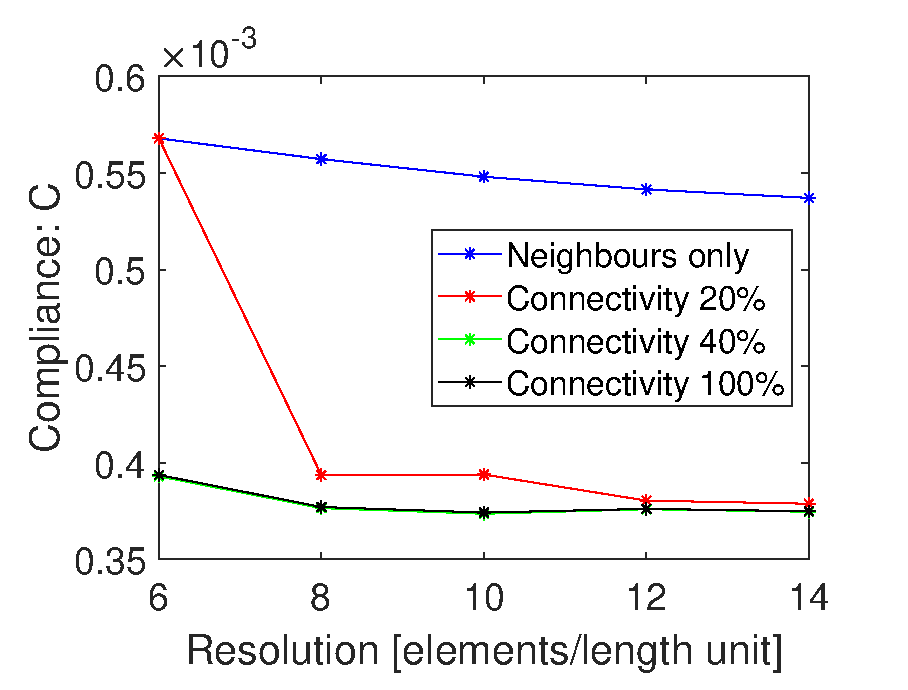
\includegraphics[trim=.0cm .0cm .0cm .0cm, clip=true,width=1\linewidth]{Figures/Plots/Comp_res_plot.eps}
\caption{}
\label{fig:com_res}
\end{wrapfigure}
Optimization was run on the structure of varying resolutions of grid ranging from 6 to 14 elements per length unit. \Cref{fig:com_res} compares the compliance for the different variations of resolutions and connectivity of the nodes.
The connectivity is given either as "Neighbours only" or as a percentage. Neighbours only means that the nodes are only connected to the immediate node in horizontal, vertical and diagonal direction and the percentage describes how far apart two connecting nodes are compared to the size of the total structure.
The results indicate that it is a great structural advantage to have the nodes connected to more than just the immediate neighbours. \Cref{fig:com_res} shows little difference in compliance for higher resolution grids when comparing the different connectivity percentages. This comes down to the connectivity being given as a percentage of the structure length, i.e. increasing the resolution also increases the amount of element-connections for each node.
\squeezeup
\squeezeup
\paragraph{4.2}
Increasing the penalization factor, $p$, results in a structure with fewer (but more dense) active elements, which is evident by comparing \cref{fig:14x14p15} to \cref{fig:14x14p1}. 
\Cref{tab:Sub4_pen_comp} presents the optimized structure's compliance from a fully connected 14x14 node grid with penalty factors ranging from 1 to 1.5. The results shows that the compliance increases with the penalization factor as the intermediate element densities becomes less stiff, effectively constraining the optimization algorithm. In conclusion, increasing $p$ results in a simpler structure, but at the loss of stiffness (compliance increases).

\vspace{2mm}
\begin{table}[h!]
    \centering
    \caption{Comparing a 14x14 node structure optimized with different penalization factors.}
    \begin{tabular}{@{}llllllll@{}}
    \toprule
   Penalization factor, $p$   & 1.0 & 1.1 & 1.2 & 1.3 & 1.4 & 1.5 \\ 
    Compliance, $C$  $[10^{-3}]$  & 0.375 & 0.397 & 0.405 & 0.417 & 0.436 & 0.453 \\ 
    \bottomrule
    \end{tabular}
    \label{tab:Sub4_pen_comp}
\end{table}
\vspace{4mm}
\begin{figure}[h!]
    \centering
\begin{subfigure}[t]{.45\textwidth}
    \centering
    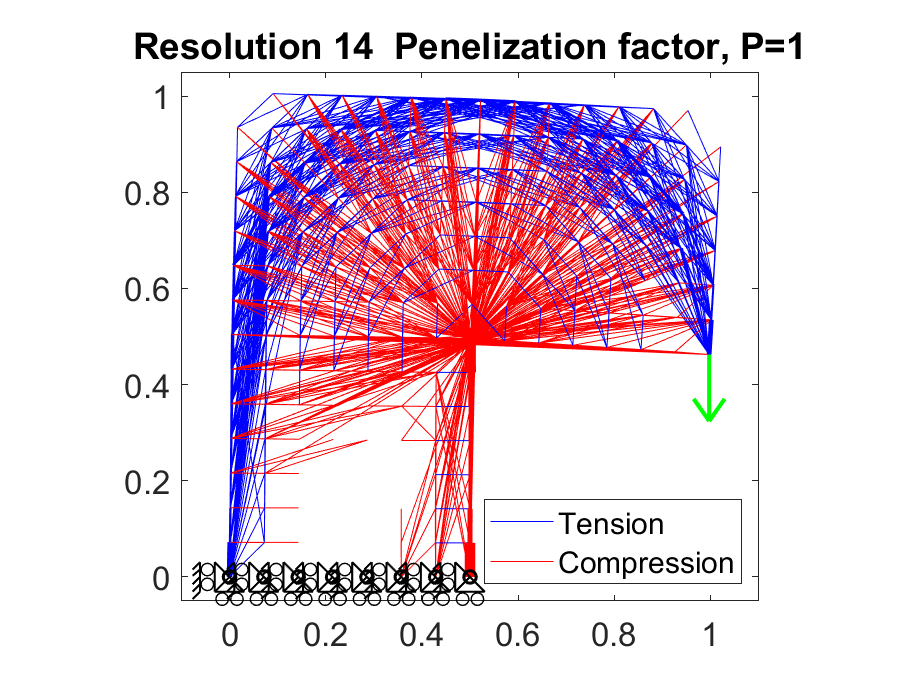
\includegraphics[trim=.0cm .0cm .0cm .0cm, clip=true,width=1\linewidth]{Figures/Plots/flex14x14c100Ex42_p=1-0.eps}
    \caption{}
    \label{fig:14x14p1}
\end{subfigure}
\begin{subfigure}[t]{.45\textwidth}
    \centering
    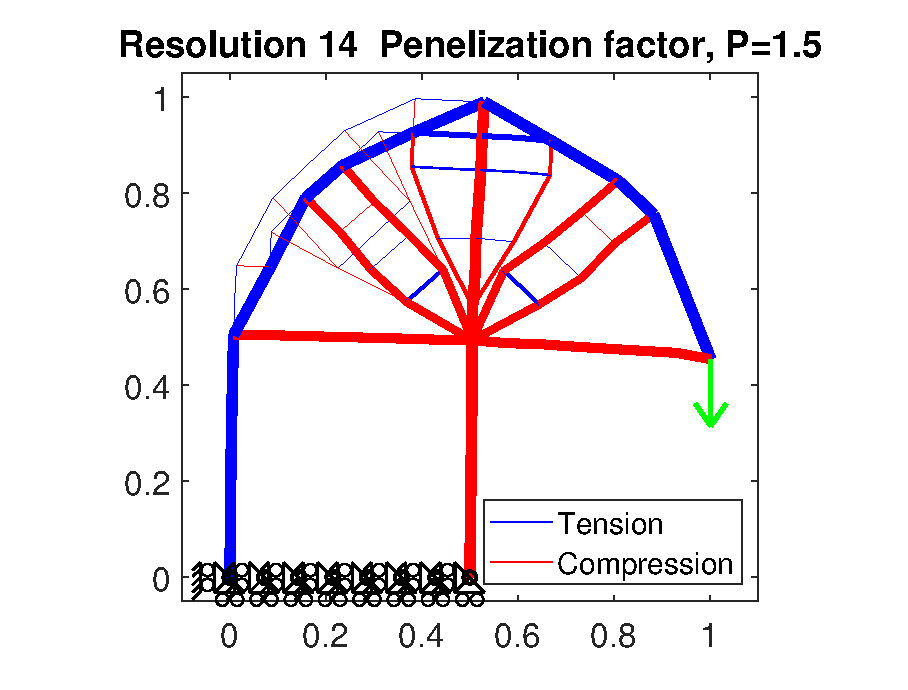
\includegraphics[trim=.0cm 0.0cm .0cm .0cm, clip=true,width=1\linewidth]{Figures/Plots/flex14x14c100Ex42_p=1-5.eps}
    \caption{}
    \label{fig:14x14p15}
\end{subfigure}
\caption{ (a) Structure using $p=1$.  (b) Structure using $p=1.5$}
\end{figure}

\paragraph{4.3}
The record from the competition was beat with the structure using any penalization factor as shown in \cref{tab:Sub4_pen_comp}. Comparing with the competition, this optimization code has the advantage of being able to change the relative element density, $\rho$ for each element. For the structures using a higher penalization factor the densities move towards either $\rho \approx 0$ or $1$, which leads to a structure closer to one that could be used in the competition. 
